\section{Results}

\subsection{Transformation Functions} 

\begin{figure}[H]
    \centering
    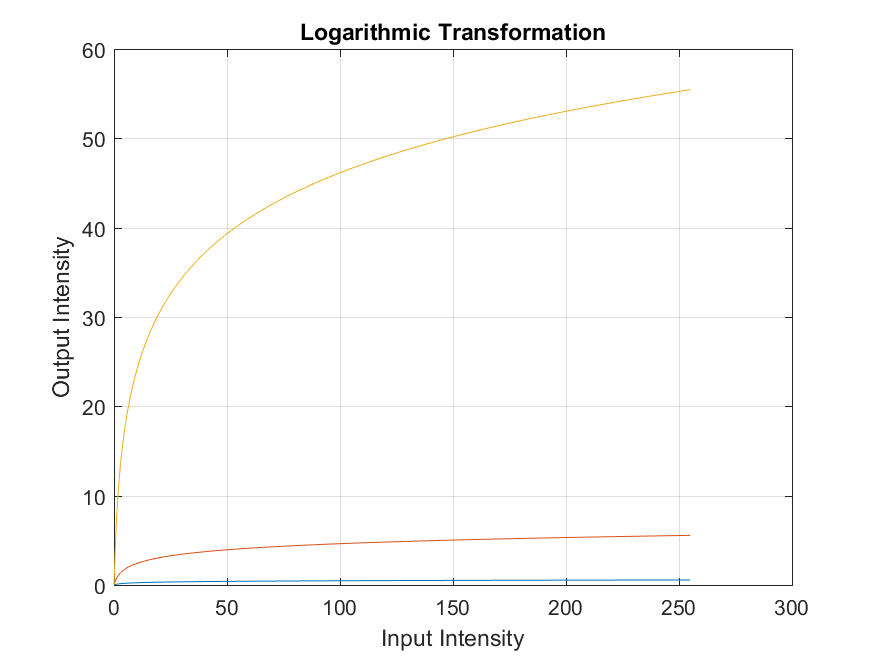
\includegraphics[scale=0.8]{logarithmic}
    \caption{Logarithmic Transfer Function}
\end{figure}

\begin{figure}[H]
    \centering
    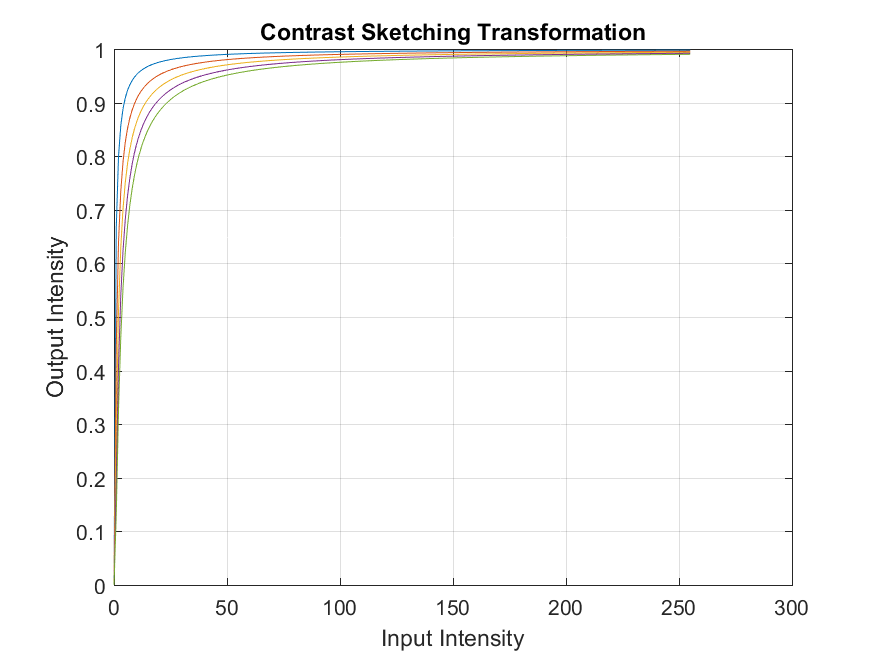
\includegraphics[scale=0.8]{contrast_stretch}
    \caption{Contrast Sketch Transfer Function}
\end{figure}

\subsection{Constant Offset}

\begin{figure}[H]
    \centering
    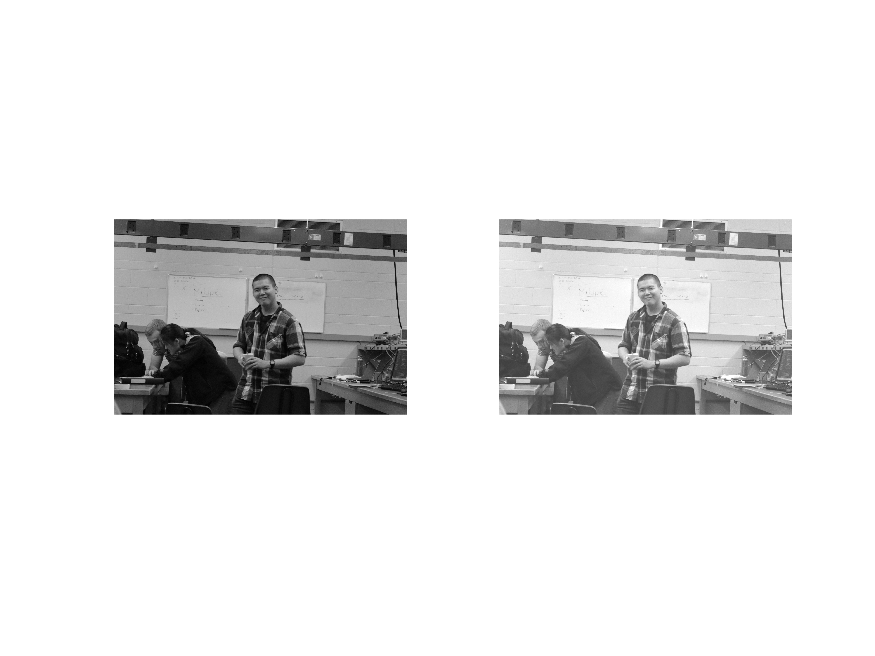
\includegraphics[scale=0.8]{twoPeters}
    \caption{Added a constant offset to peter}
\end{figure}

\subsection{Negative Image}

\begin{figure}[H]
    \centering
    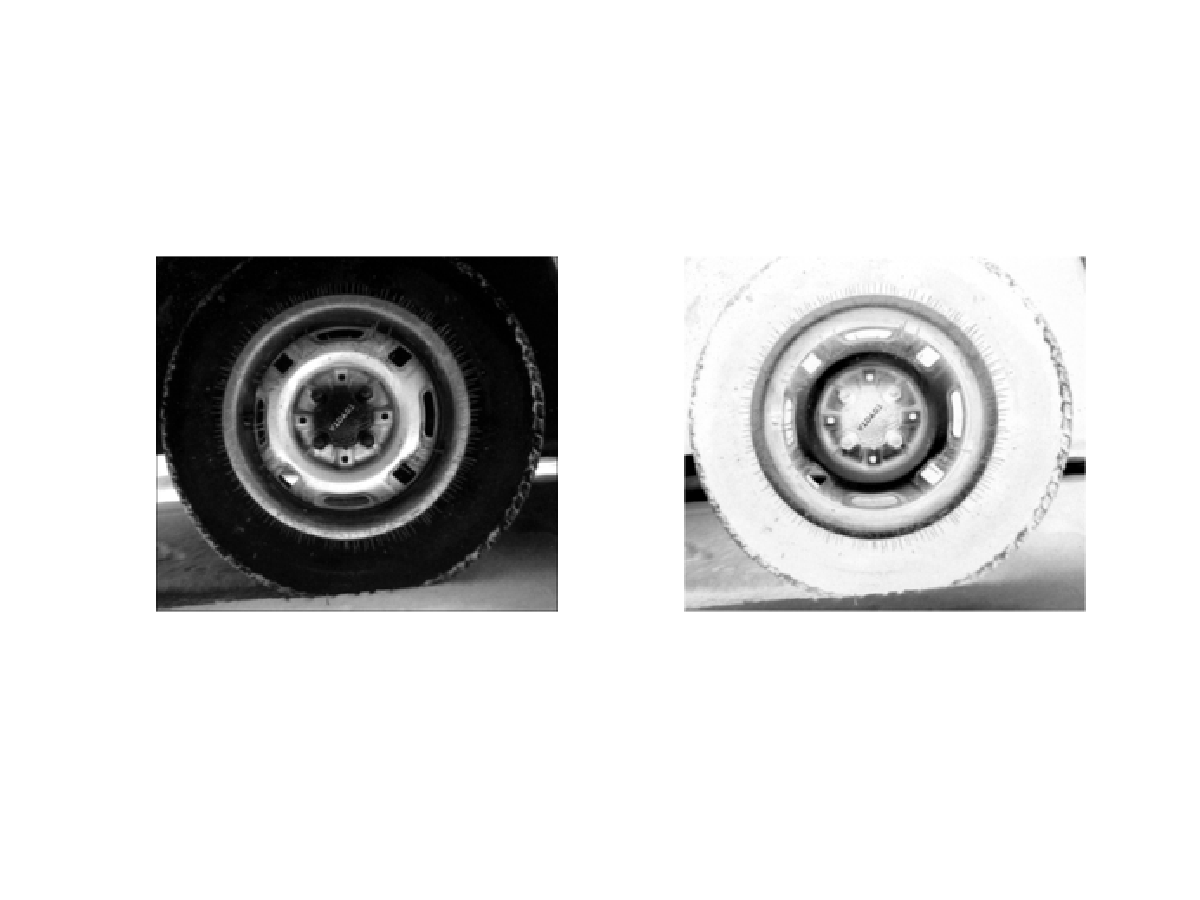
\includegraphics[scale=0.8]{tire_neg}
    \caption{Negative Image of Tire}
\end{figure}

\subsection{Gamma Transform}

\begin{figure}[H]
    \centering
    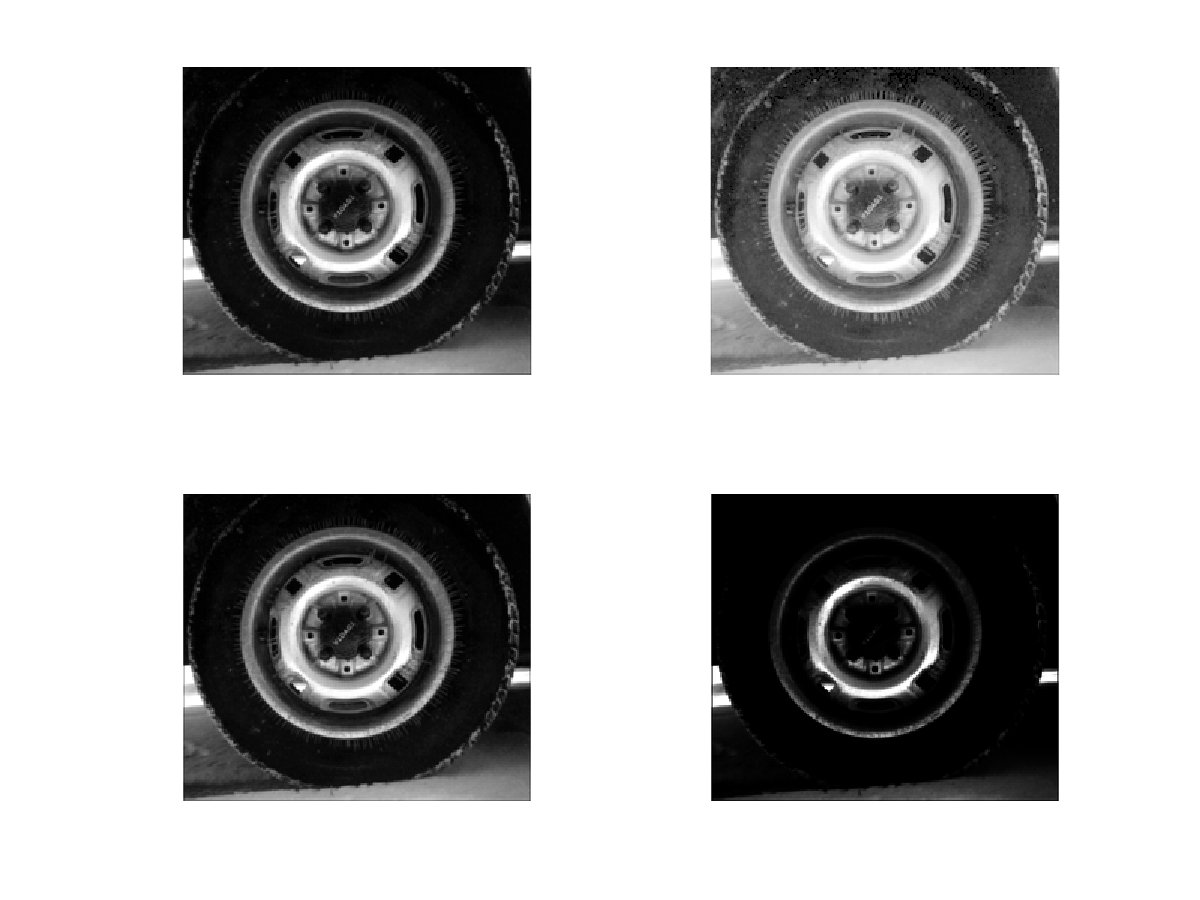
\includegraphics[scale=0.8]{tire_gamma}
    \caption{Gamma transformations of tire}
\end{figure}

\subsection{Logarithmic Transfrom}

\begin{figure}[H]
    \centering
    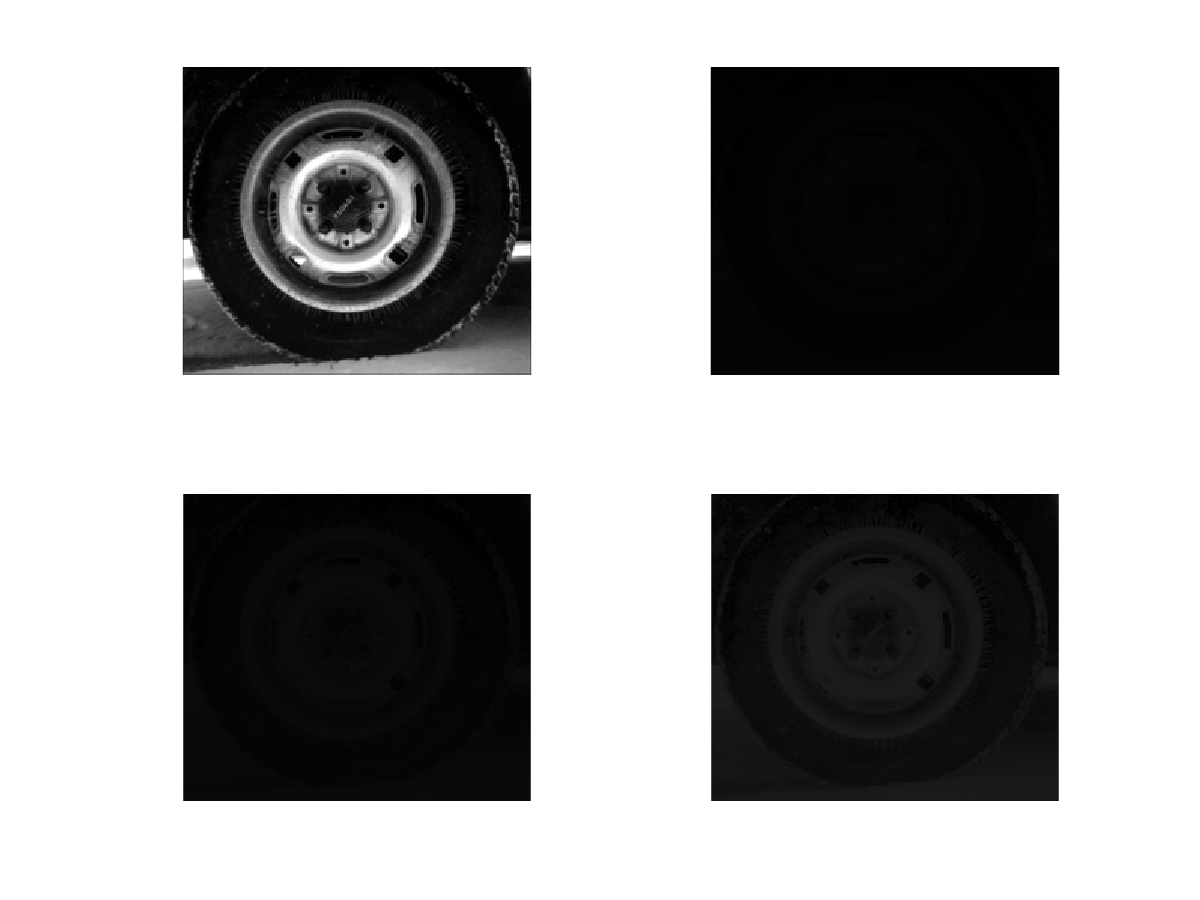
\includegraphics[scale=0.8]{tire_log}
    \caption{Logarithmic transformations of tire}
\end{figure}

\subsection{Piecewise Transform}

\begin{figure}[H]
    \centering
    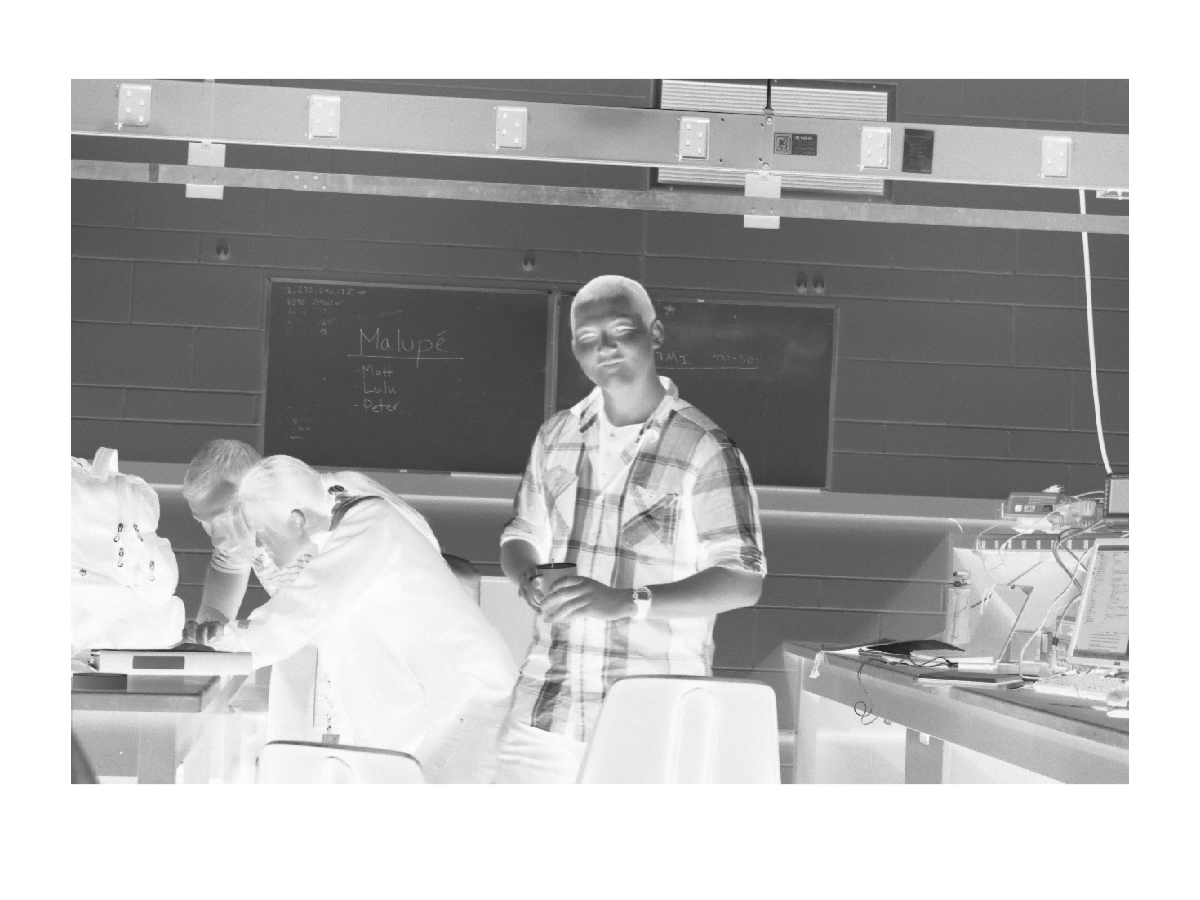
\includegraphics[scale=0.8]{peter_neg}
    \caption{Negative Transformation of Peter}
\end{figure}

\begin{figure}[H]
    \centering
    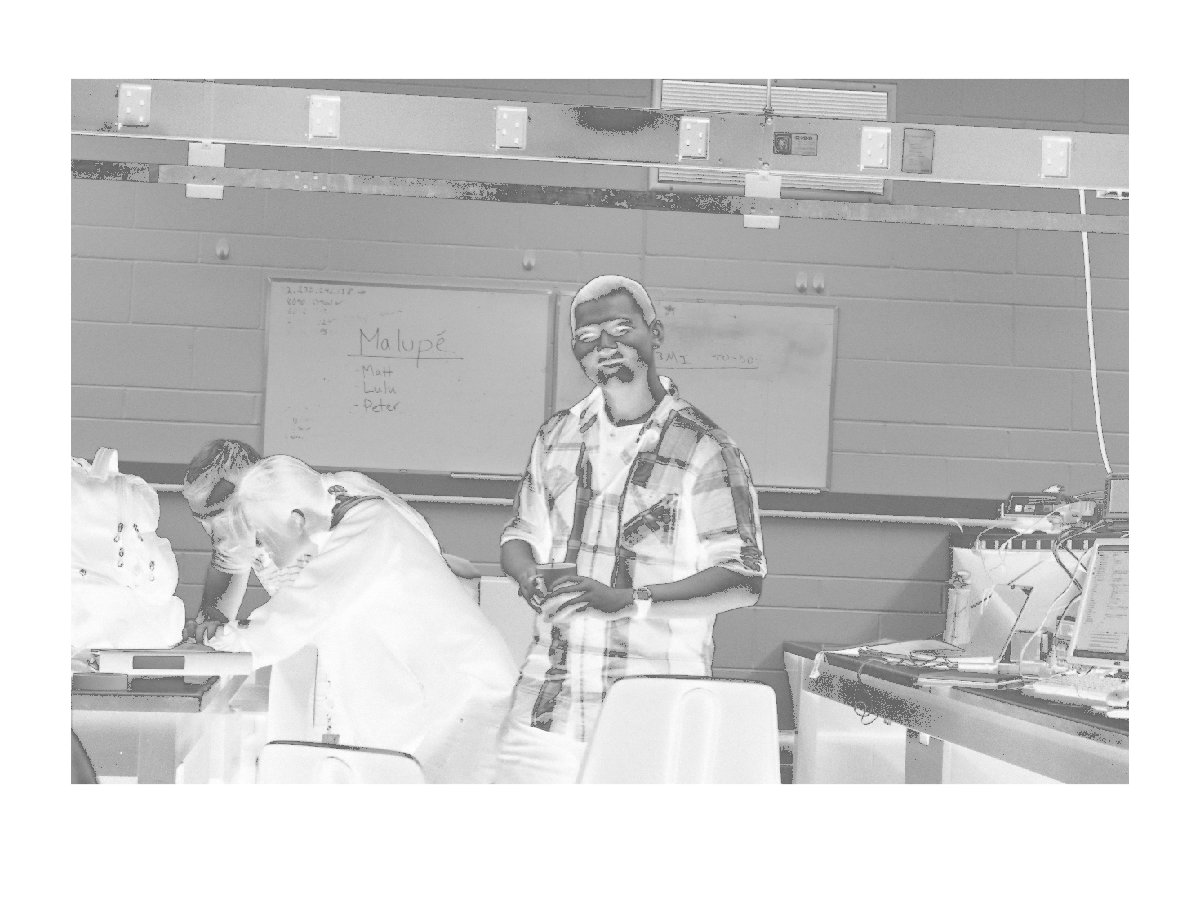
\includegraphics[scale=0.8]{peter_partial}
    \caption{negT transform of peter with threshold = 100}
\end{figure}

\subsection{Translation}

\begin{figure}[H]
    \centering
    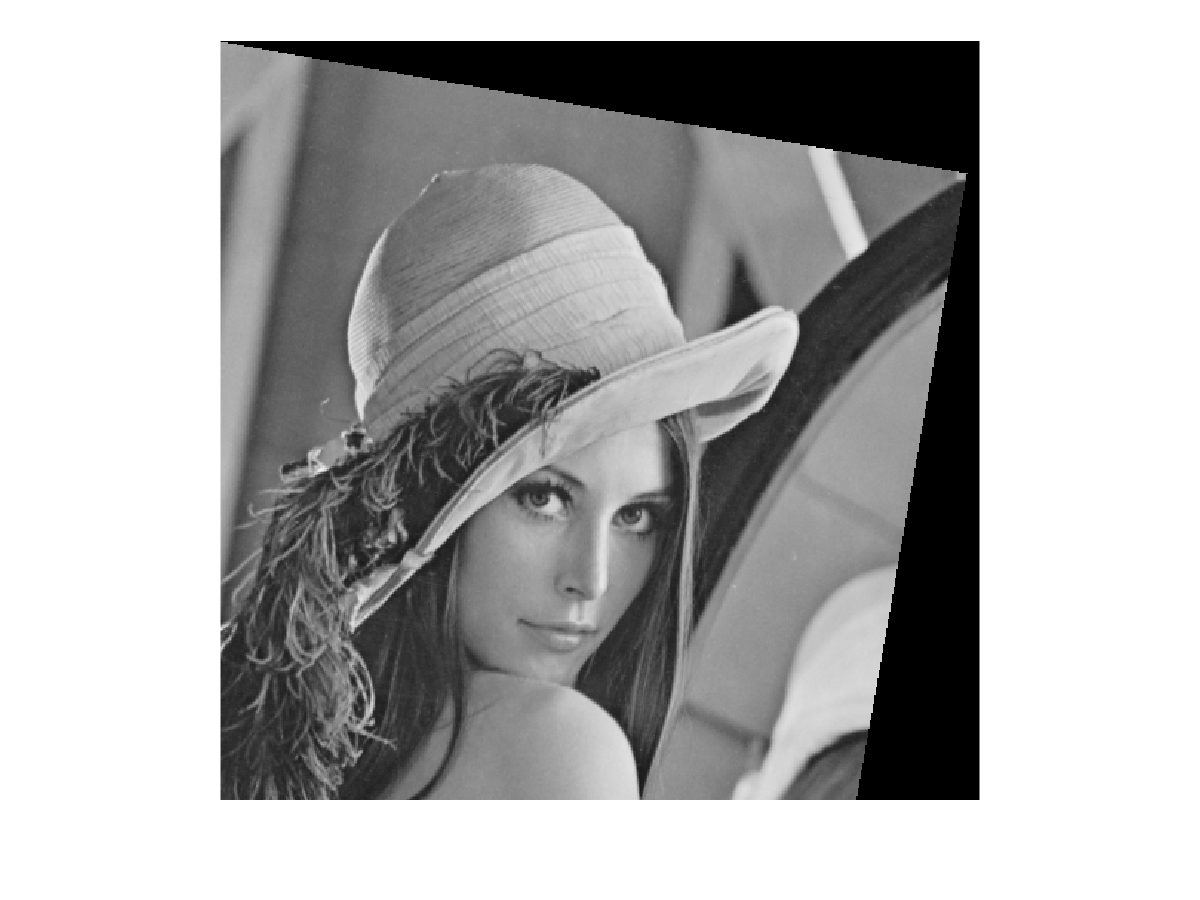
\includegraphics[scale=0.8]{lena_rot1}
    \caption{lena rotated 10 degrees clockwise}
\end{figure}

\begin{figure}[H]
    \centering
    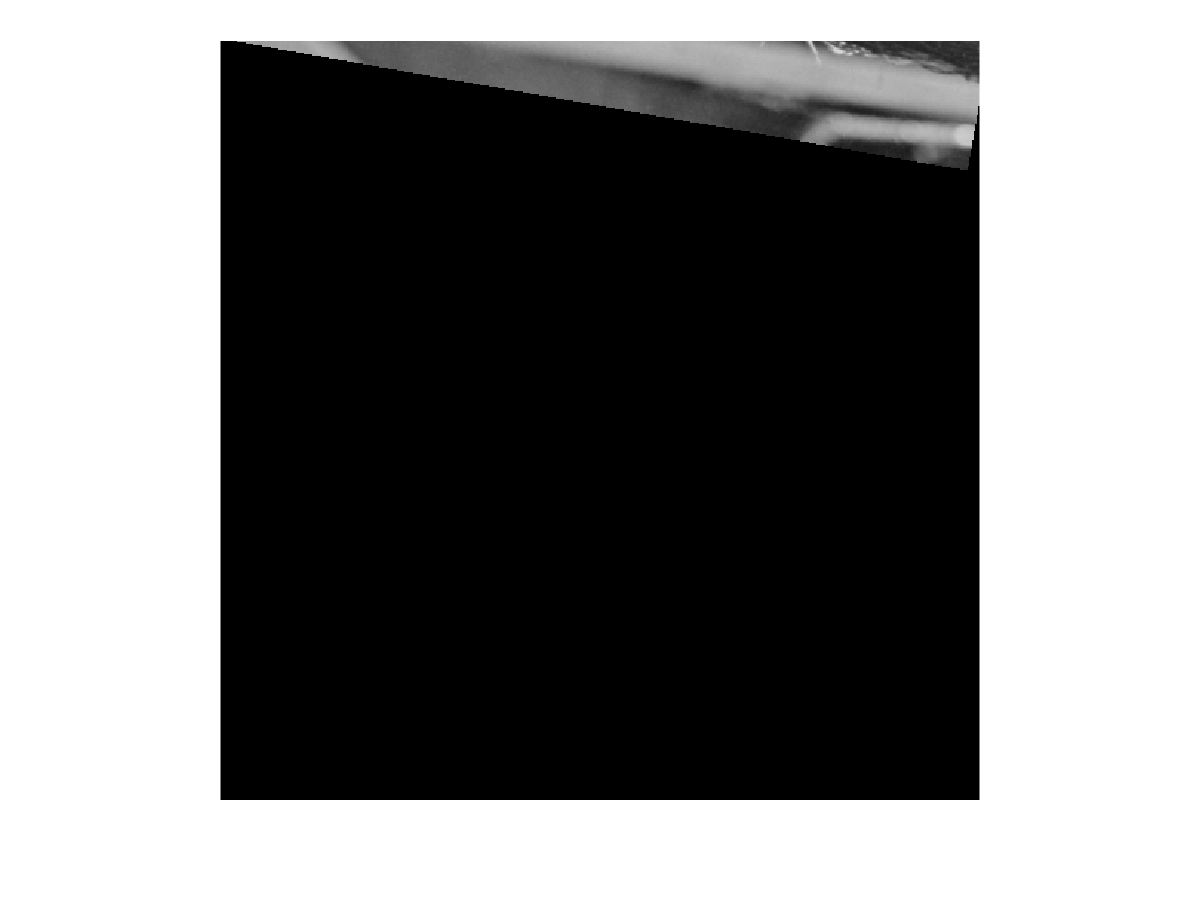
\includegraphics[scale=0.8]{lena_rot2}
    \caption{lena rotated 80 degrees counterclockwise}
\end{figure}
